\documentclass[accentcolor=tud9c,colorbacktitle,inverttitle,landscape,german,presentation,t]{tudbeamer}
\usepackage{amstext}
\usepackage{amsmath}
\usepackage{graphicx}
\usepackage{multicol}
\usepackage{mathtools}
\usepackage{subfigure}
\usepackage[ngerman,english]{babel}
\usepackage[utf8]{inputenc}
\usepackage{colortbl}
\usepackage{adjustbox}

\begin{document}

\title{\"Ubung 11 - Gruppe 142}
\subtitle{Visual Computing - Informationsvisualisierung}


\author[Johannes Beck, Christian Eilers, Robin Menzenbach, Martin Steinborn]{Johannes Beck, Christian Eilers, Robin Menzenbach, Martin Steinborn}


\date{\today}

\begin{titleframe}
\end{titleframe}

\section{Aufgabe 1}
	\begin{frame}
		\frametitle{Aufgabe 1}
		\begin{itemize}
			\item[1] Raw Data (Bild \textbf{C})
			\item[2] Data Tables (Bild \textbf{B})
			\item[3] Visual Structures (Bild \textbf{A})
			\item[4] Views (Bild \textbf{D})
		\end{itemize}
	\end{frame}
\section{Aufgabe 2}
\begin{frame}
	\frametitle{Aufgabe 2}
	Fehler in der Visualisierung:
	\begin{itemize}
	\item Ungenauigkeit in der Legende/Beschreibung: Es wird nicht genannt, um was für Verkaufszahlen es sich handelt. Daher könnte sowohl von Autos, Einzelteilen wie auch Merchandise-Artikeln usw. die Rede sein.
	\item Die 3D Perspektive verzerrt die Wahrnehmung der dargestellten Werte.
	\end{itemize}
\end{frame}
\section{Aufgabe 3}
\begin{frame}
	\frametitle{Aufgabe 3}
	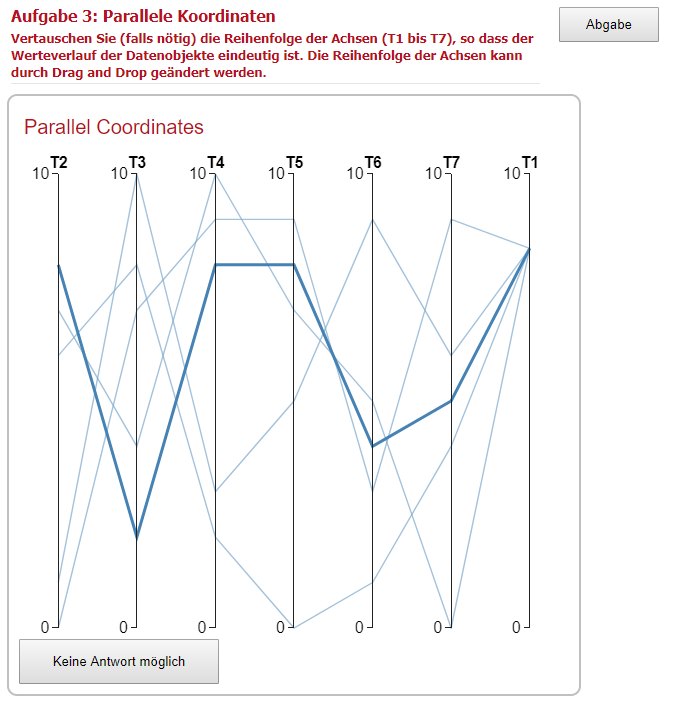
\includegraphics[height=\textheight]{ex11_3.png}
\end{frame}
\section{Aufgabe 4}
\begin{frame}
	\frametitle{Aufgabe 4 - a)}
	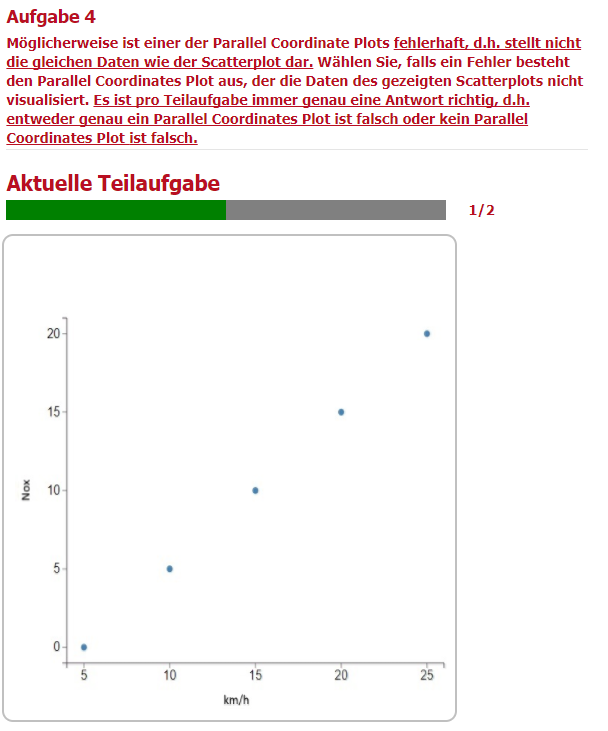
\includegraphics[width=0.45\linewidth]{ex11_4a_1.png}
	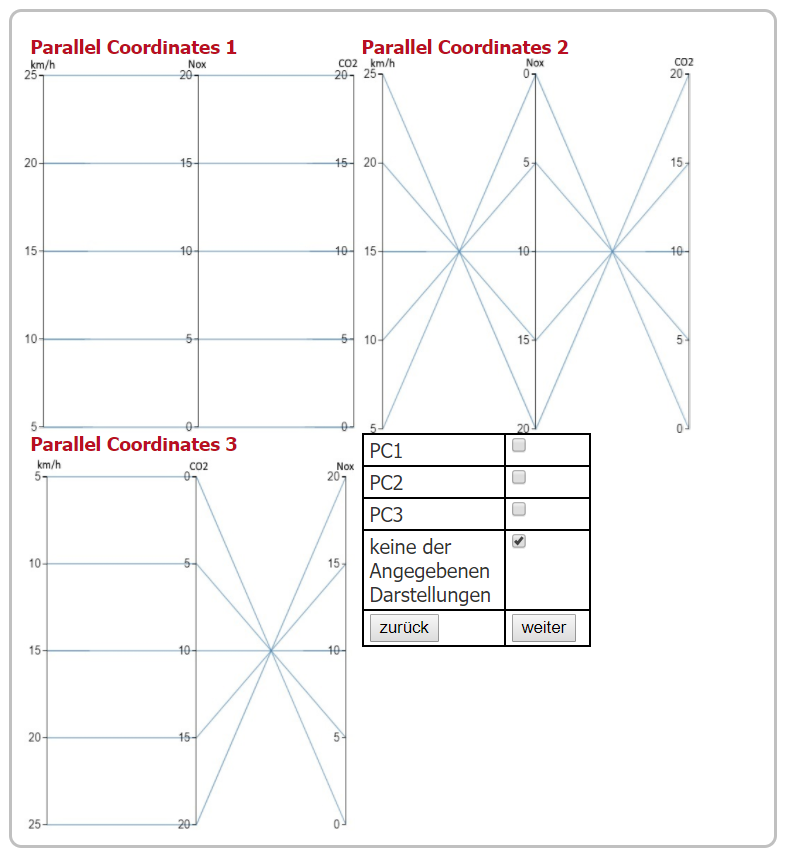
\includegraphics[width=0.45\linewidth]{ex11_4a_2.png}
\end{frame}
\begin{frame}
	\frametitle{Aufgabe 4 - b)}
	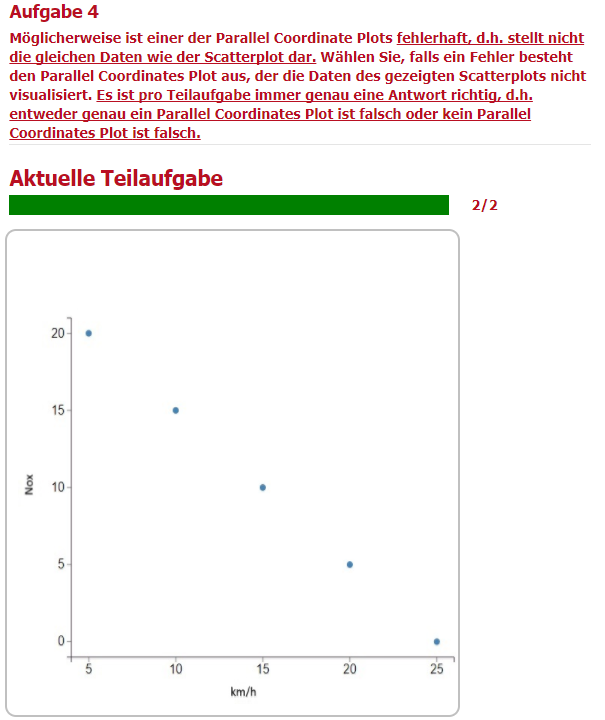
\includegraphics[width=0.45\linewidth]{ex11_4b_1.png}
	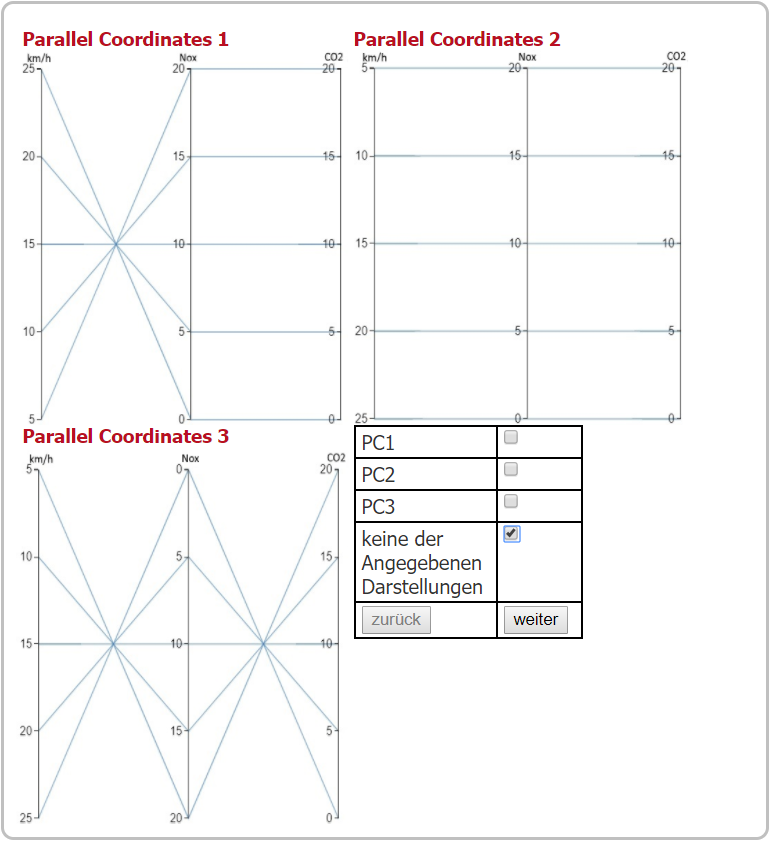
\includegraphics[width=0.45\linewidth]{ex11_4b_2.png}
\end{frame}
\section{Aufgabe 5}
\begin{frame}
	\frametitle{Aufgabe 5 - a)}
	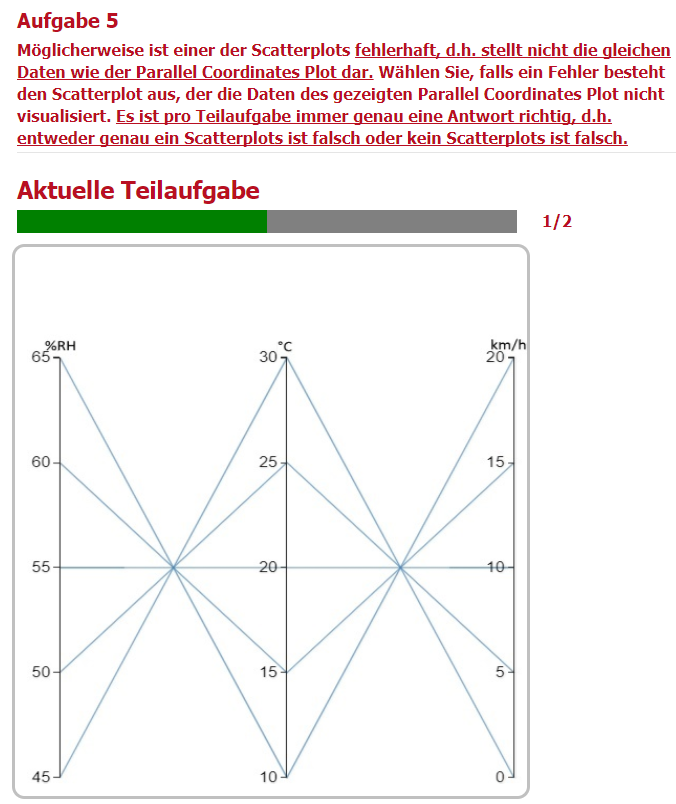
\includegraphics[width=0.45\linewidth]{ex11_5a_1.png}
	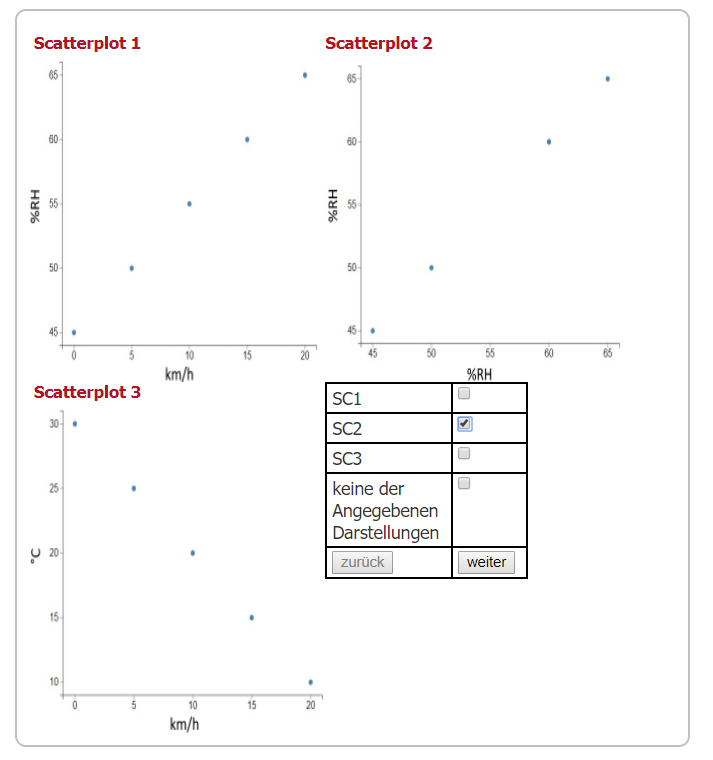
\includegraphics[width=0.45\linewidth]{ex11_5a_2.png}
\end{frame}
\begin{frame}
	\frametitle{Aufgabe 5 - b)}
	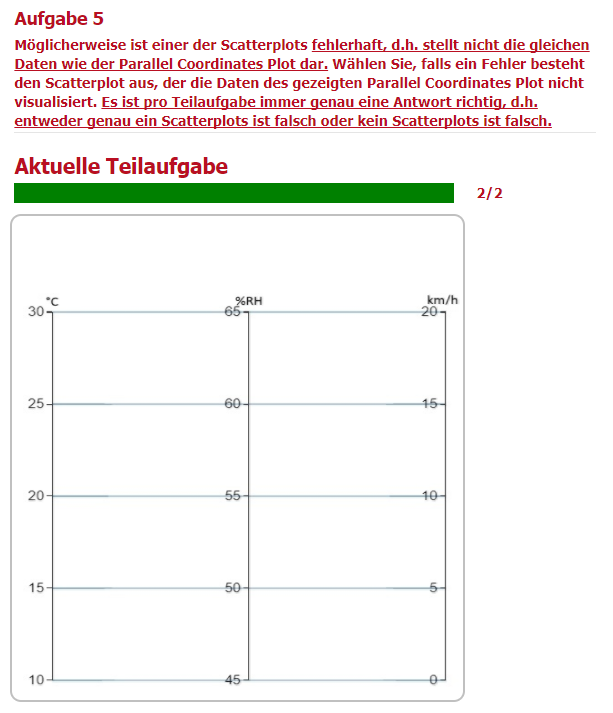
\includegraphics[width=0.45\linewidth]{ex11_5b_1.png}
	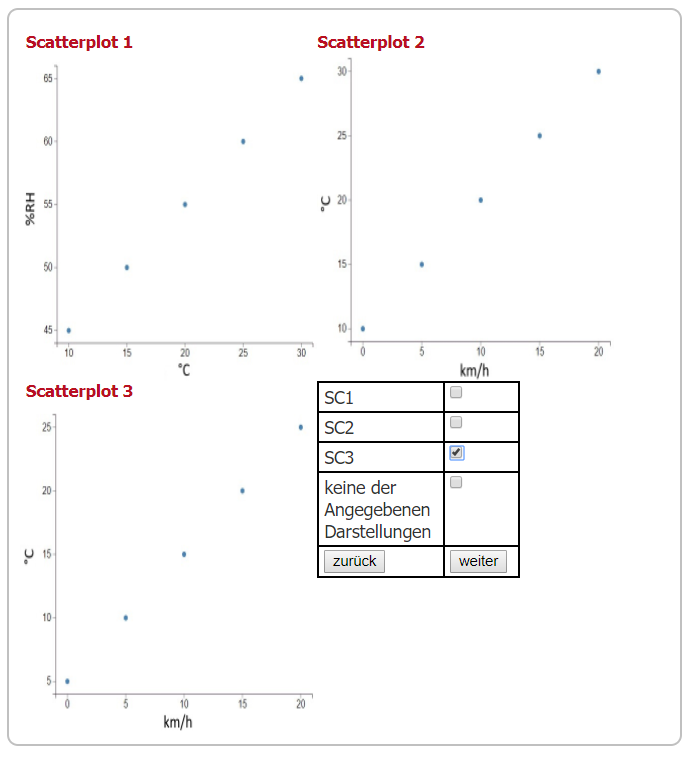
\includegraphics[width=0.45\linewidth]{ex11_5b_2.png}
\end{frame}
\section{Aufgabe 6}
\begin{frame}
	\frametitle{Aufgabe 6 - a)}
	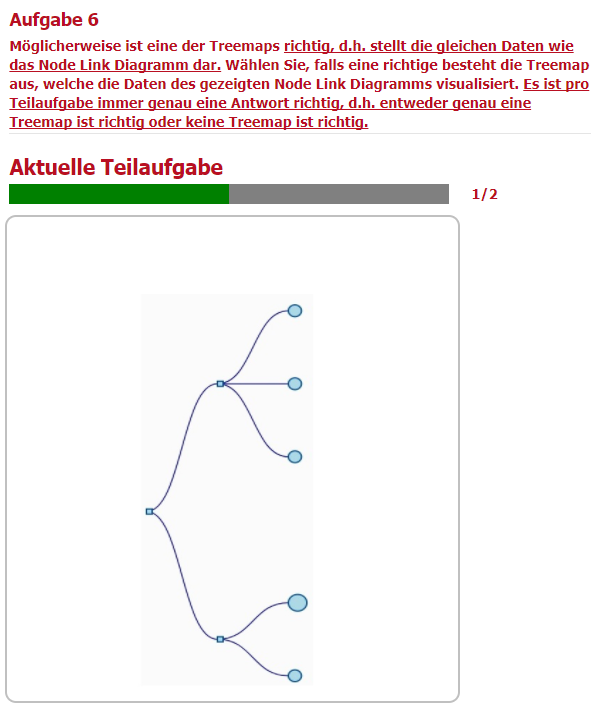
\includegraphics[width=0.45\linewidth]{ex11_6a_1.png}
	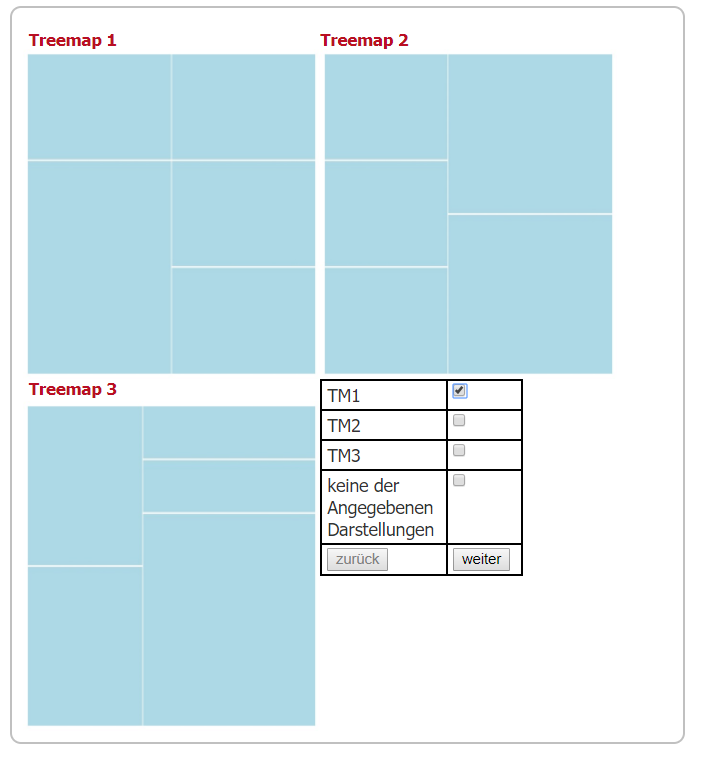
\includegraphics[width=0.45\linewidth]{ex11_6a_2.png}
\end{frame}
\begin{frame}
	\frametitle{Aufgabe 6 - b)}
	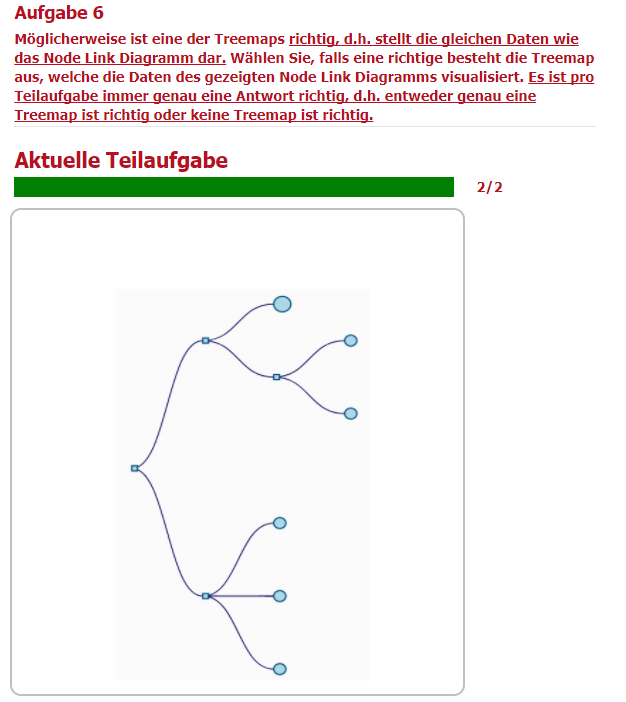
\includegraphics[width=0.45\linewidth]{ex11_6b_1.png}
	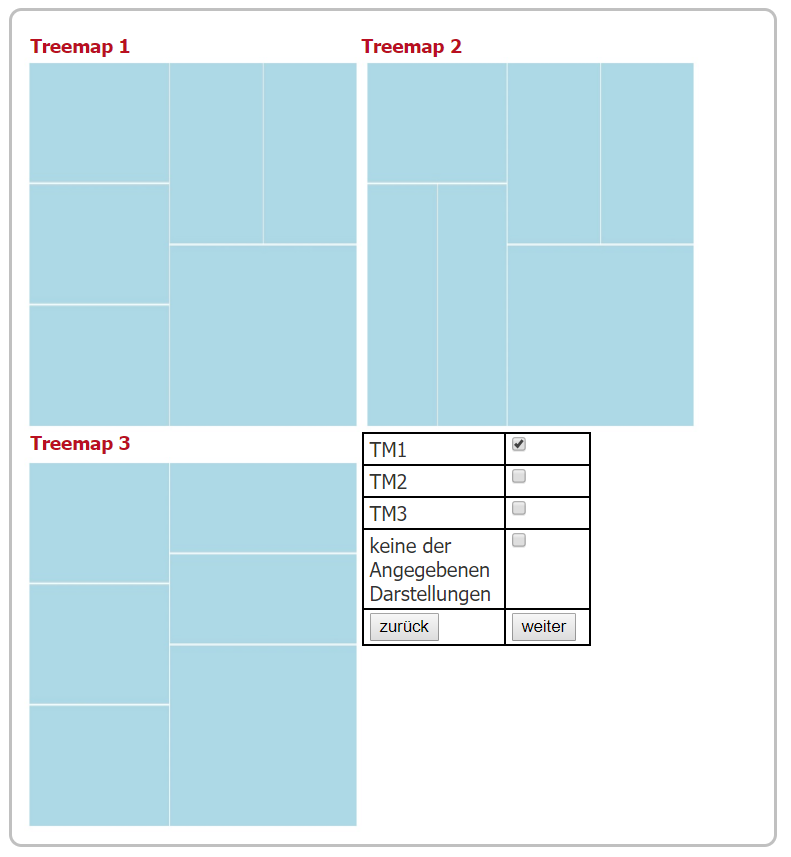
\includegraphics[width=0.45\linewidth]{ex11_6b_2.png}
\end{frame}
\end{document}
